\documentclass[10pt,a4paper]{book}
\usepackage[utf8]{inputenc}
\usepackage[french]{babel}
\usepackage[T1]{fontenc}
\usepackage{amsmath}
\usepackage{amsfonts}
\usepackage{amssymb}
\author{Hexanome: 4105\\\\Alexis Andra\\Jolan Cornevin\\Mohamed Haidara\\Alexis Papin\\Robin Royer\\Maximilian Schiedermeier\\David Wobrock}
\title{Compte Rendu DevOO}
\usepackage{graphicx}
\usepackage{xcolor}
\usepackage[hidelinks]{hyperref}
\usepackage{natbib}
\usepackage{listings}
\usepackage{color}
\definecolor{lightgray}{rgb}{.95,.95,.95}
\definecolor{darkgray}{rgb}{.4,.4,.4}
\definecolor{purple}{rgb}{0.65, 0.12, 0.82}
\lstdefinelanguage{JavaScript}{
  keywords={typeof, new, true, false, catch, function, return, null, catch, switch, var, if, in, while, do, else, case, break, done, fi, elif, for},
  keywordstyle=\color{blue}\bfseries,
  ndkeywords={class, export, boolean, throw, implements, import, this},
  ndkeywordstyle=\color{darkgray}\bfseries,
  identifierstyle=\color{black},
  sensitive=false,
  comment=[l]{//},
  morecomment=[s]{/*}{*/},
  commentstyle=\color{purple}\ttfamily,
  stringstyle=\color{black}\ttfamily,
  morestring=[b]',
  morestring=[b]"
}
\lstset{
   language=JavaScript,
   frame=single,
   extendedchars=true,
   basicstyle=\footnotesize\ttfamily,
   showstringspaces=false,
   showspaces=false,
   numbers=left,
   numberstyle=\footnotesize,
   numbersep=9pt,
   tabsize=2,
   breaklines=true,
   showtabs=false,
   captionpos=b,
   backgroundcolor=\color{lightgray},
}

\makeindex
\begin{document}
\maketitle
\tableofcontents 
\chapter{Capture et Analyse des besoins}
\section{Planning prévisionnel du projet}
Le planning prévisionnel du projet s'est dérouillé en trois étapes. Au début on a identifié les stations nécessaires pour réaliser le projet systématiquement. Cette découpage en missions réalisables est exprimé par la liste suivante:
\begin{itemize}
	\item{Planning previsionnel du projet (3.0 h)}
	\item{Analyse du modèle (3.0h)}
	\item{Conception du modèle (2.5 h)}
	\item{Analyse des \textit{CU}s, conception des \textit{diagrammes des sequence} (3.5 h)}
	\item{Description textuelle des \textit{CU}s (4.0 h)}
	\item{Implémentation des classes représentant donnes des \textit{XMLs} (1.5 h)\footnote{La planification d'une heure et demi peut apparaitre insuffisant pour implémenter un modèle. Au moment du conception de l'architecture, le modèle était compris comme une ensemble des Java Beans. La réalisation des algorithmes était prevu dans le package contrôleur.}}
	\item{Conception d'IHM (prototype) (8.0 h)}
	\item{Conception d'IHM (précise) (8.0 h)}
	\item{Spécification '\textit{événements utilisateur} (4.0 h)}
	\item{Conception du diagramme \textit{États-transitions} (6.0h)}
	\item{Implémentation du serialiseur / deserialiseur (8.0 h)}
	\item{Spécification des Interfaces du package contrôleur (5.0 h)}
	\item{Spécification des Interfaces du package vue (3.0 h)}
	\item{Spécification des Interfaces du package modele (5.0 h)}
	\item{Conception de diagramme des classes du package controleur (6.0 h)}
	\item{Conception de diagramme des classes du package vue (3.0 h)}
	\item{Conception de diagramme des classes du package modele (6.0 h)}
	\item{Implémentation des observateurs qui notifient la vue (4.0 h)}
	\item{Réalisation de l'IHM (package vue) (20 h)}
	\item{Mock implémentation des classes du package controleur (3.5 h)}
	\item{Conception et réalisation des tests unitaires (20 h)}	
	\item{Conception et réalisation des tests fonctionnels (20 h)}
	\item{Implémentation du package contrôleur (30 h)}
	\item{Implémentation du package vue (20 h)}
	\item{Implémentation du package modèle (10 h)}
	\item{Rétro-génération des diagrammes classes a partir du code (3.0 h)}
	\item{Redaction du glossaire (2.0 h)}
\end{itemize}
~\\Deuxièmement on a essayé de trouver toutes les dépendances entre les missions prévus. Le but de cette démarche était de pouvoir paralléliser les développements. La graphique suivant montre le déroulement prévisionnel du projet et également qui était le responsable prévu pour chaque étape.

\begin{figure}[ht!]
    \centering
    \scalebox{.65}{\input{der.pdf_tex}}
    \caption{Dépendances et déroulement prévisionnel du projet}
\end{figure}

~\\Dans la troisième et dernière étape, on a essayé d'estimer le temps nécessaire pour réaliser ces taches en utilisant redmine.
\begin{figure}
    \centering
    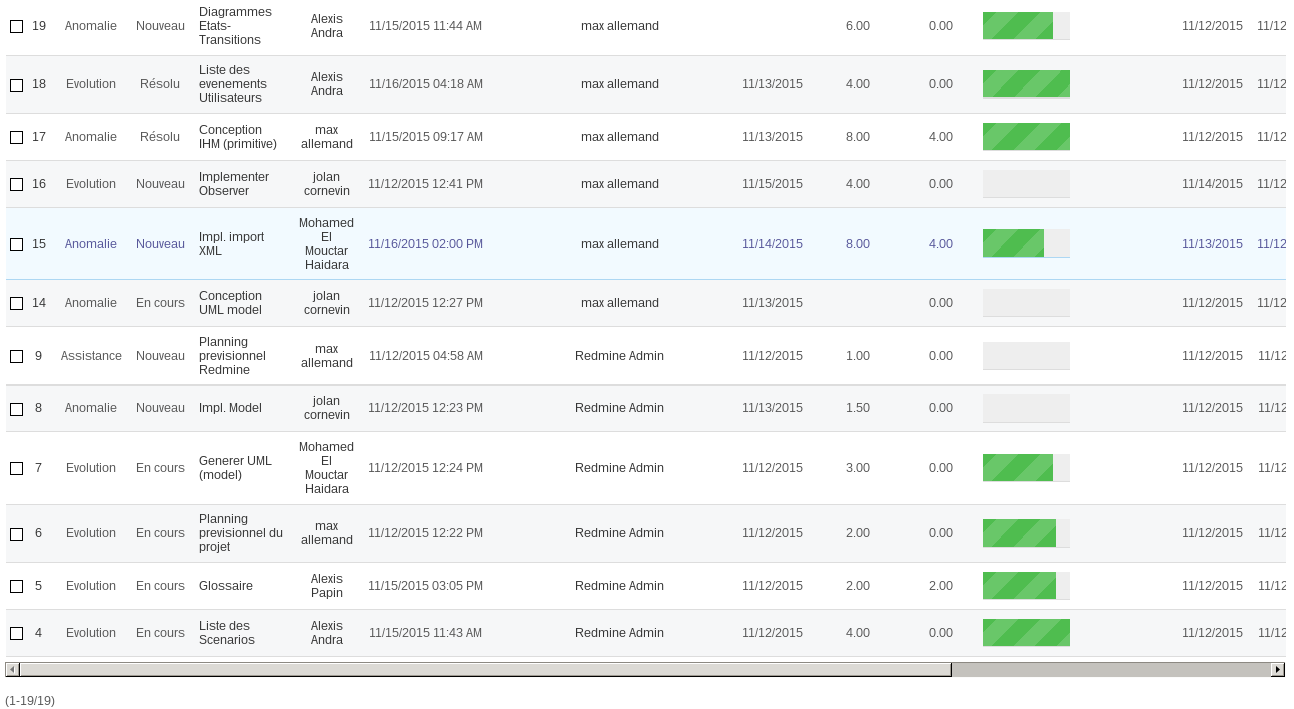
\includegraphics[scale=0.25]{redmine.png}
%http://www.dplot.com/examples/surface-plot-phong-shading.png
    \caption{Capture d'écran de la gestion du projet avec redmine} 
\end{figure}

\section{Modèle du domaine}
\section{Glossaire}
\section{Diagramme de cas d'utilisation}
\section{Description textuelle structurée des cas d'utilisation}
\chapter{Conception}
\section{Liste des événements utilisateur et diagramme États-Transitions}
\section{Diagrammes des packages et de classes}
\section{Document expliquant les choix architecturaux et design patterns utilisés}
\section{Diagramme des sequence du calcul de la tournée a partir d'une demande de livraison}
\chapter{Implémentation et tests}
\section{Code du prototype et des tests unitaires}
\section{Documentation JavaDoc du code}
\section{Diagramme de packages et de classes rétro-générés à partir du code}
\chapter{Bilan}
\section{Planning effectif du projet}
Le planning prévisionnel nous a aide beaucoup de réaliser ce projet dans une maniéré bien pensée. La connaissance des dépendances entre les modules nous permettait d'éviter que un développeur sera bloque et de réaliser les taches dans la bonne ordre.\\
Comme le relevé en haut montre, le planning prévisionnel était suffisamment précis pour ce que concerne la planification et conception. Par contre on a pas réussi à réaliser les implémentations dans le temps prévu. Il y a 
\section{Bilan humain et technique}
\subsection{Bilan humain}
Coordonner le projet et notamment distribuer les taches dans l'équipe était un devoir délicat. D'un cote un but était la parallélisation les fils de développement le plus possible. D'autre part il y avait beaucoup des dépendances entre les étapes prévus. C'est pour ça qu'au début du projet la priorité était d'identifier une procédure raisonnable qui permettait d'identifier les stations critiques. Comme je n'étais jamais avant en charge d'une équipe assez nombreuse et puissant je dois admettre que d'abord j'avais sous-estimé ce défi.\\ Le résultat de cet effort nous a bien permit de profiter au maximum des ressources humaines. Néanmoins il était important de tenir tout l' équipe en courant en ce que regarde les développements qui se sont déroule dans les cotes divers du projet en parallèle. En particulier la convention de bien commenter son code en combinaison avec une communication fréquente nous ont permis de maitriser cette mission.\\Personnellement je le trouvait éprouvant de trouver une raisonnable granularité pour la distribution des taches ouverts dans l'équipe. Si une charge est trop petit, on risque de perdre du temps en expliquant le contexte. Aurait elle pu réalisé plus rapide directement par la personne qui s'en a déjà occupe? Sinon, quand les taches sont trop complexe on risque qu'un développeur sera bloqué et exclu des événements qui se passent concurremment. Comme la section avant a relevé, la nombre des heures passes sur le project par développeur n'est pas parfaitement équilibré. Cependant on ne doit pas oublier que les chiffres ne correspondent pas toujours précisément au travail réalisé. Notamment le temps passe avec planification, communication et réflexion n'est pas facile à mesurer. Pour ça il me semble plus avéré d'évaluer l'équipe comme un entité indivisible.\\
Parlant de l'équipe, on peut résumer que on était enchanté de pouvoir observer la réalisation de nos conceptions. Même s'il y avait parfois des défis qu'on n'avait pas prévu, l'équipe était toujours motivé de discuter et trouver la meilleure solution possible.
\subsection{Bilan technique}
Pour réaliser ce projet nous avons profite d'une grande variété des techniques. Au but de permettre à chaque développeur de travailler avec son IDE préféré, nous avons décidé de ne pas garder les fichiers de gestion d'IDE dans le répertoire git. Grâce a çà, nous avons réussi à travailler avec des IDEs \textit{NetBeans}, \textit{Eclipse} et \textit{IntelliJ} en même temps. Concernant les fichiers de conception nous avons également utilisé plusieurs outils:
\begin{itemize}
	\item{La conception des diagrammes de classes était réalisé avec le logiciel \textit{UMLet} \footnote{http://www.umlet.com/}. Les fichiers utilisés par ce logiciel étaient également partagé dans le répertoire git.}
	\item{Pour tous les autres diagrammes on a profite des outils en ligne, particulièrement \textit{Draw.io}, disponible sur \textit{Google Drive}.}
	\item{Pour automatiquement charger les librairies dont on avait besoin, on a intégré \textit{Apache Maven}. On pourrait argumenter que l'intégration de Maven n'était pas forcement nécessaire, car il y avait seulement quatre dépendances. Néanmoins son intégration était très confortable pour l'équipe parce qu'on a jamais perdu du temps en ressoudant les dépendances soulevé par un collègue.}
	\item{Les tests fonctionnels et unitaires étaient réalises en utilisant \textit{JUnit}. Même si les tests ont contribue beaucoup à trouver et résoudre des erreurs, on aurait encore pu intensifier leur intégration. On a suivi le conseil de jamais laisser un développeur tester son propre code. Quoique ce soit en général une bonne pratique, on avait parfois pas assez de communication entre un auteur d'un classe et le testeur. Ça peut causer que les tests écrit ne peuvent pas passer, car ils n'utilisent pas les interfaces la manière prévu.}
\end{itemize}
Finalement on peut résumer que même si il s'agitait d'un projet complexe et qu'on avait pas beaucoup du temps pour le réaliser, nous avons choisi les bonnes outils. Celles ci nous avons permis d'avancer rapidement et créer un produit fiable.
\appendix{}
\end{document}